\documentclass[a4paper,12pt]{article}
\usepackage[utf8]{inputenc}
\usepackage[cm,empty]{fullpage}
\usepackage[T2A]{fontenc}
\usepackage[english, russian]{babel}
\usepackage{amssymb,amsmath,amsxtra,amsthm}
\usepackage{proof}
\usepackage[pdftex]{graphicx}
\usepackage{wrapfig}

\usepackage[left=2cm,right=2cm,
    top=1cm,bottom=1cm,bindingoffset=0cm]{geometry}

\renewcommand{\leq}{\leqslant}
\renewcommand{\geq}{\geqslant}


\newcommand{\iiff}{\Longleftrightarrow}
\renewcommand{\iff}{\Leftrightarrow}
\newcommand{\nothing}{\varnothing}


\newcommand{\NN}{\mathbb{N}}
\newcommand{\ZZ}{\mathbb{Z}}
\newcommand{\Q}{\mathbb{Q}}
\newcommand{\A}{\mathbb{A}}
\newcommand{\R}{\mathbb{R}}
\renewcommand{\C}{\mathbb{C}}

\renewcommand{\phi}{\varphi}
\newcommand{\eps}{\varepsilon}

\newcounter{z}


\newcommand{\zs}{\refstepcounter{z}\vskip 10pt\par\noindent
\fbox{\textbf{12.\arabic{z}}} }

\newcommand{\z}{\refstepcounter{z}\vskip 20pt\noindent
\fbox{\textbf{\arabic{z}}} }

\renewcommand{\date}{{\bf 11 ноября 2020}} %Дата занятия

\newcommand{\dif}
{
------------------------------------------------------------------------------------------------------------------------------------------------------
}

\newcommand{\HSEhat}{
\vspace*{-0pt}
\noindent
\setcounter{z}{0}
\vspace*{-10pt}
\begin{wrapfigure}[2]{l}{5pt}
\vspace*{-25pt}
\hspace*{-20pt}

\includegraphics[scale=0.18]{img/HSE_LOGO.png}
\end{wrapfigure}
\vspace{-20pt}


{\bf \phantom{\date}  \large \hfill Дискретная математика: \hfill \normalsize \date}

\vspace{5 pt}
{\bf \large \hfill  множества и логика.\hfill }

\vspace{15 pt}
\centerline{ \large  Примеры решения задач.}



\vspace*{10pt}
\setcounter{z}{0}

}

\begin{document}

\HSEhat

\z  Выполнено ли равенство для любых множеств $A$, $B$ и $C$?\\

$$(A \backslash C) \cup(B \backslash C)=(A \cup B)\triangle C.$$

Если равенство верно, то докажите его. Если не выполнено, то приведите контрпример.\\

{\bf Решение.} Равенство не выполнено. В качестве контрпримера подходят, например, множества $A=\{1,2\},\ B=\{2,3\},\ C=\{3,4\}$. Для таких множеств элемент $4$ множества $C$ содержится в множестве, соответствующей правой части равенства, но не лежит в левой части равенства.

Действительно, $4 \in C$ и $4 \notin (A \cup B)$ $\Longrightarrow$ $4 \in (A \cup B)\triangle C.$

Но $4 \notin (A \backslash C)$ и $4 \notin (B \backslash C)$ $\Longrightarrow$ $4 \notin (A \backslash C) \cup(B \backslash C).$\\


{\bf Комментарий к решению.} Понять, как может выглядеть контрпример, можно построив диаграммы Эйлера-Венна.

\centerline{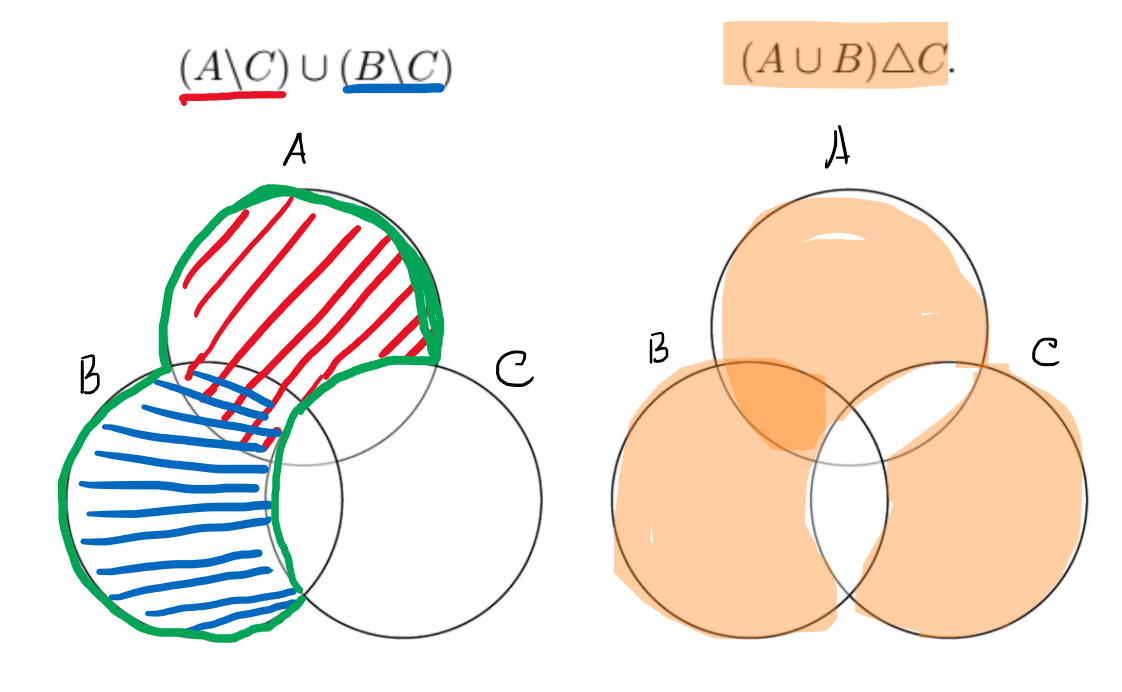
\includegraphics[scale=0.3]{img/exmpl.png}}

\z  Для какого из названий животных ложно высказывание: <<Заканчивается на согласную букву $\wedge$ (В слове $7$ букв $\rightarrow \neg$(Третья буква согласная))>>?
\\

1) верблюд \qquad 2) страус \qquad 3) кенгуру \qquad 4) леопард\\

{\bf Решение.} Упростим высказывание. Для этого выведем вспомогательную формулу $$a\rightarrow \neg b=\neg (a \wedge b). \quad (*)$$
Формула (*) следует из таблицы истинности:
\\

\begin{tabular}{|c|c|c|c|}
\hline$a$ & $b$ & $a\rightarrow \neg b$ & $\neg (a \wedge b)$ \\
\hline 0 & 0 & 1 & 1 \\
\hline 0 & 1 & 1 & 1 \\
\hline 1 & 0 & 1 & 1 \\
\hline 1 & 1 & 0 & 0 \\
\hline
\end{tabular}
\\

Обозначим высказывания

a$=$<<Заканчивается на согласную букву>>, 

b$=$<<В слове $7$ букв>>,

c$=$<<Третья буква согласная>>.

Получаем формулу $a\wedge (b \rightarrow \neg c$). Из (*) следует:

$$a\wedge (b \rightarrow \neg c)=a\wedge \neg( b \wedge c).$$

Нам необходимо указать те слова, для которых это высказывание ложно. Высказывание
$a\wedge \neg( b \wedge \neg c)$ ложно когда его отрицание $\neg (a\wedge \neg( b \wedge \neg c))$ истинно. Используя законы де Моргана (были на занятии)

$$\neg (a\wedge \neg( b \wedge c))=\neg a \vee \neg\neg( b \wedge c)=\neg a \vee ( b \wedge c).$$

Иными словами, подходят те слова, для которых верно или $\neg a$, или $( b \wedge c)$.

Поскольку $\neg a$=$\neg$ <<Заканчивается на согласную букву>> = <<Заканчивается на гласную букву>>, то осталось найти те слова, у которых последняя буква гласная, или те, в которых $7$ букв и третья согласная.

Такими являются  1) верблюд и 3) кенгуру.\\


{\bf Ответ:} 1) верблюд и 3) кенгуру.

\z Пусть $A=\{ x\ |\ x=k^2,\ k\in \ZZ \}$ (множество всех целых чисел), $B=\{12,0,4,2,6,8,10\}, C= \{ 3,1,9,7,5,11\}$. Для каких $x\in A$ предикат <<$\neg(x \in B)\rightarrow (x \in C)$>> обращается в истину?\\

{\bf Решение.} Упорядочим множество $B=\{12,0,4,2,6,8,10\}=\{0,2,4,6,8,10,12\}$ и $C= \{ 3,1,9,7,5,11\}=\{ 1,3,5,7,9,11\}$. Нетрудно заметить, что $B$ -- множество четных чисел в промежутке от $0$ до $12$, а $C$ -- множество нечетных чисел в промежутке от $0$ до $12$.\\

Теперь упростим предикат <<$\neg (x \in B) \rightarrow (x \in C)$>> $=\neg b(x)\rightarrow c(x)$, где $b(x)$ и $с(x)$ обозначают предикаты $(x \in B)$ и $(x \in C)$.

Согласно формуле (*) из предыдущего задания и законам де Моргана $$\neg b(x)\rightarrow c(x)=\neg \left(\neg b(x) \wedge \neg c(x)\right)= b(x) \vee  c(x).$$

Как известно (было на занятии), предикату $b(x) \vee  c(x)$ соответствует множество $B\cup C$. Таком образом, осталось найти элементы из $A$, которые удовлетворяют предикату (вопрос задачи), т.е. лежат в $B\cup C$. Иными словами, найти множество $A\cap (B\cup C)$. 

Множество $A$ --- полные квадраты (числа, которые являются квадратами целого числа: $0,1,4,9,16,\ldots $). Множество $B\cup C$ -- объединение четных и нечетных чисел в промежутке от $0$ до $12$, т.е. все натуральные числа от $0$ до $12$. Получаем, что предикату удовлетворяют в точности все квадраты, не превосходящие $12$, а именно $0,1,4,9$.\\

{\bf Ответ:} $0,1,4,9$.


\end{document}